\documentclass[tikz]{standalone}
\usetikzlibrary{positioning}
\usetikzlibrary{arrows.meta}
\tikzset{
  bnode/.style = {align=center, inner sep=1pt, text centered, circle, white, font=\sffamily\bfseries, 
    fill=orange, text width=1.5em},
}
\begin{document}
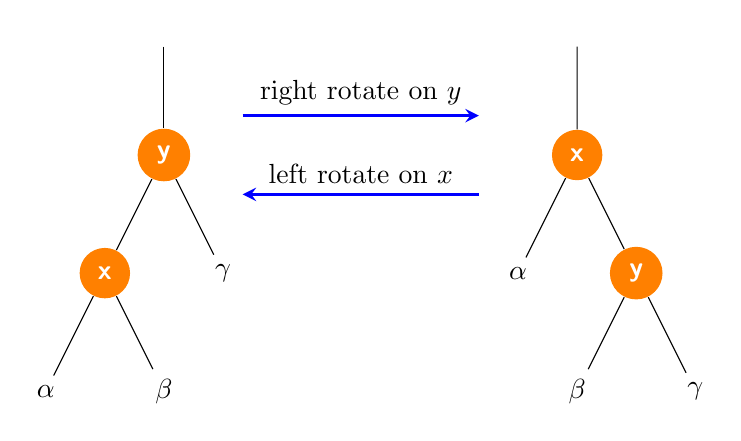
\begin{tikzpicture}
    \node (lefttree) {}
        child { node [bnode] {y}
            child {node [bnode] {x}
                child {node {$\alpha$}}
                child {node {$\beta$}}
            }
            child {node {$\gamma$}}
            };
    
    \draw [-stealth, line width=0.4mm, draw=blue](1,-1) -- (4,-1)node[midway,above,shape=rectangle,draw=none]{right rotate on $y$};

    \draw [stealth-, line width=0.4mm, draw=blue](1,-2) -- (4,-2)node[midway,above,shape=rectangle,draw=none]{left rotate on $x$}; 

    \node (right) [right=5cm of lefttree] {}
            child { node [bnode] {x}
                child {node {$\alpha$}}
                child {node [bnode] {y}
                    child {node {$\beta$}}
                    child {node {$\gamma$}}
                    }
                };
\end{tikzpicture}
\end{document}

